\documentclass{article}
\setlength{\parskip}{5pt} % esp. entre parrafos
\setlength{\parindent}{0pt} % esp. al inicio de un parrafo
\usepackage{amsmath} % mates
\usepackage[sort&compress,numbers]{natbib} % referencias
\usepackage{url} % que las URLs se vean lindos
\usepackage[top=15mm,left=20mm,right=20mm,bottom=25mm]{geometry} % margenes
\usepackage{hyperref} % ligas de URLs
\usepackage{graphicx} % poner figuras
\usepackage[spanish]{babel} % otros idiomas

\author{Claudia Lizeth Hern\'andez Ram\'irez} % author
\title{Homework 0} % titulo
\date{\today}

\begin{document} % inicia contenido

\maketitle % cabecera

\begin{abstract} % resumen
  \centering
  Es un documento para comenzar con el manejo de Overleaf.
\end{abstract}

\section{Introducci\'{o}n}\label{intro} % seccion y etiqueta


Este texto nos servir\'a como una gu\'ia para realizar nuestros reportes de las tareas durante el semestre. 



\section{Desarrollo}\label{desarrollo} % Desarrollo de la tarea
Debemos comprender como insertar ecuaciones: \eqref{equ}:
\begin{equation}
  f(x) = 2 \sin(x) - \int_0^\infty \frac{1}{1 + x} \text{d}x.
  \label{equ}
\end{equation}
Como citar fuentes \citep{ejemplo} .
\textsf{Como cambiar tipos } \texttt{de letras}.\\
Como insertar im\'agenes (Una linda fotografía de uno de mis perros, Armadillo)


\section{Conclusi\'on}

En esta tarea se conoci\'o un poco sobre el manejo de la plataforma Overleaf. Seguiremos trabajando para conocer  m\'as comandos y mejorar el manejo y control del mismo.



\begin{figure} % figura
    \centering
    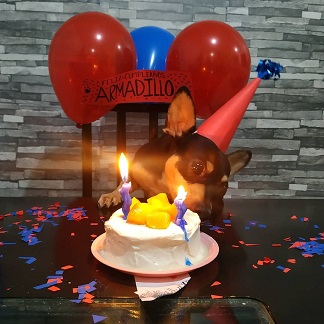
\includegraphics[width=30mm]{armadillo.jpg} % archivo
    \caption{Armadillo en su fiesta de cumpleaños \url{https://www.cumpleañosdearmadillo.es/elmundodelosperros/2020/10/20/perros/1295977576.html} con licencia CC.}
    \label{armadillo}
\end{figure}



\bibliography{referencias}
\bibliographystyle{plainnat}

\end{document}
